\chapter{Úvod}

Stavebnice \lego{ }je jedna z~nejznámějších a nejprodávanějších stavebnicí na světě. 

V~nabídce firmy \lego{ }je i~robotický set s~názvem \legoM. 

Dle oficiálních údajů se jedná historicky nejprodávanější set z~celé nabídky firmy~\cite{legoGizmodo_SalesStatistic}. 
To je také jeden z~hlavních důvodů, proč se tato práce věnuje této stavebnici. 
%To je také jeden z hlavních důvodů, proč je tato práce zaměřena na tuto stavebnici. 

Z~výše uvedených informací vyplývá, že jde pravděpodobně o~nejdostupnější robotickou stavebnici na světě (pokud pomineme platformu \arduino, která je ovšem zaměřena na jinou skupinu lidí -- lidí, kteří se nebojí elektroniky, elektronických obvodů, složitějších návrhů konstrukce, atd.).

\begin{figure}[h]
	\centering
	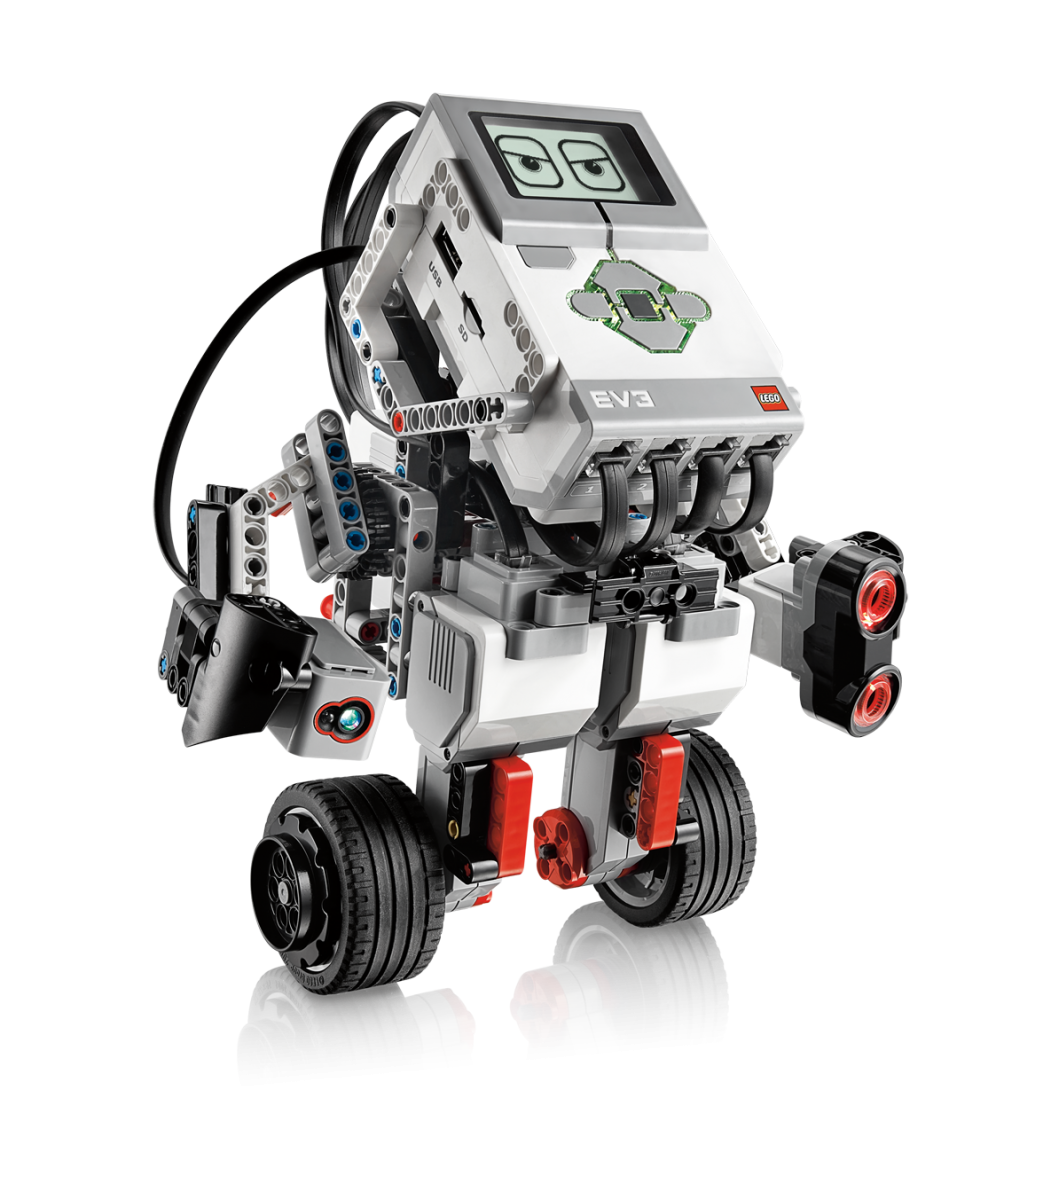
\includegraphics[width=250px]{images/lego-mindstorms-ev3_Robotics-for-Kids.png}
	\caption[\legoEV{ }-- samobalancující robot]{\legoEV{ }-- samobalancující robot\protect\footnotemark}
	\label{fig:lego-mindstorms-ev3_Robotics-for-Kids}
\end{figure}


\footnotetext{Zdroj: \url{https://www.bermotech.com/training/coding-for-teenagers-and-children/y-robotics-with-lego-mindstorm-ev3/}}

\begin{figure}[h]
	\centering
	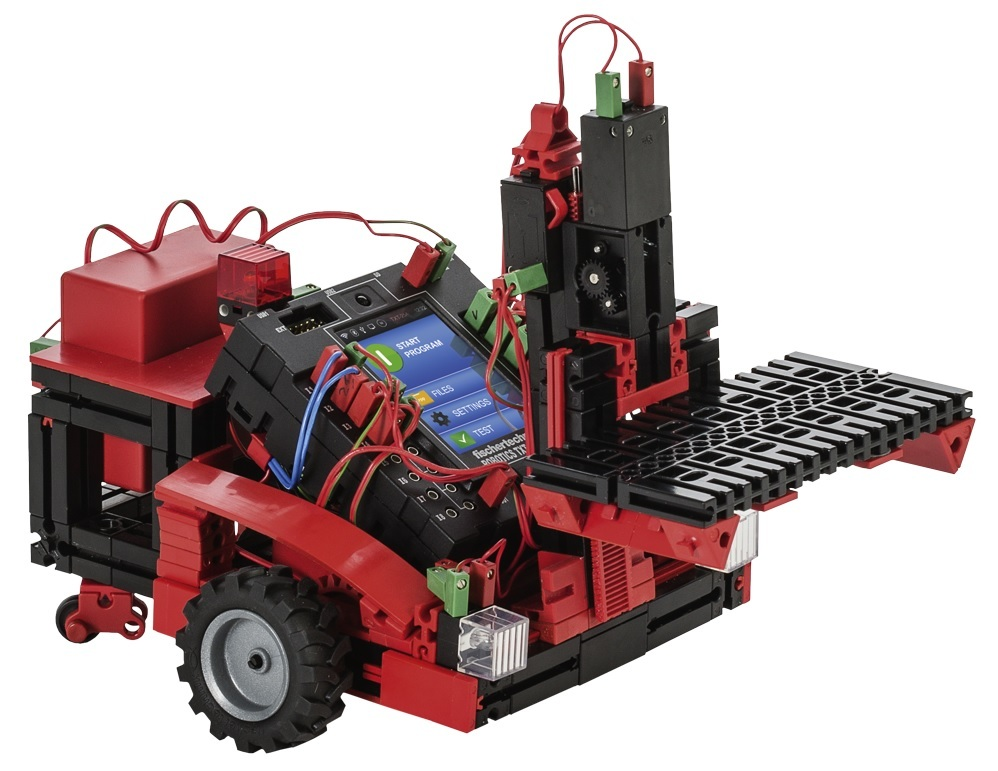
\includegraphics[width=250px]{images/fischertechnik_ROBO-TX-Explorer_02.jpg}
	\caption[Fischertechnik -- ROBO TX Explorer]{Fischertechnik -- ROBO TX Explorer\protect\footnotemark}
	\label{fig:fischertechnik_ROBO-TX-Explorer}
\end{figure}

\footnotetext{Zdroj: \url{http://www.helago-cz.cz/eshop-519143-workstation-robo-tx-training-lab-tx-explorer-146560.html}}

Existuje i mnoho podobných stavebnic~\cite{intorobotics_BestAlternativesToLegoMindstormsKits}. 
Například \fischerT prodává podobné robotické sety jako \lego{~}\cite{fischertechnik_ROBOTICS}. 

Uživateli nabízí rozsáhlejší pohled do elektroniky a~fungování jednotlivých modulů. 
Umožňuje také relativně snadno přidat vlastní moduly.
Zároveň má jednoduché grafické programovací prostředí podobně jako \lego. 
\FischerT{ }ovšem není tak rozšířen jako \legoM, protože ačkoliv nabízí v~některých ohledech více funkcí, zároveň klade větší nároky na uživatele, je podstatně dražší (základní set~\cite{fischertechnik_HelagoEshop_ROBOTICS-TXT-COMPETITION-SET} stojí cca dvakrát tolik co \legoEV{ Základní souprava}~\cite{lego_eduxeEshop_CoreSet}) a~nemá takový věhlas a~značku.

% figure + footnote -> minipage 
%src: http://www.tex.ac.uk/FAQ-ftncapt.html
% \begin{figure}[h]
% \begin{minipage}{\textwidth}
%  	\centering
% 	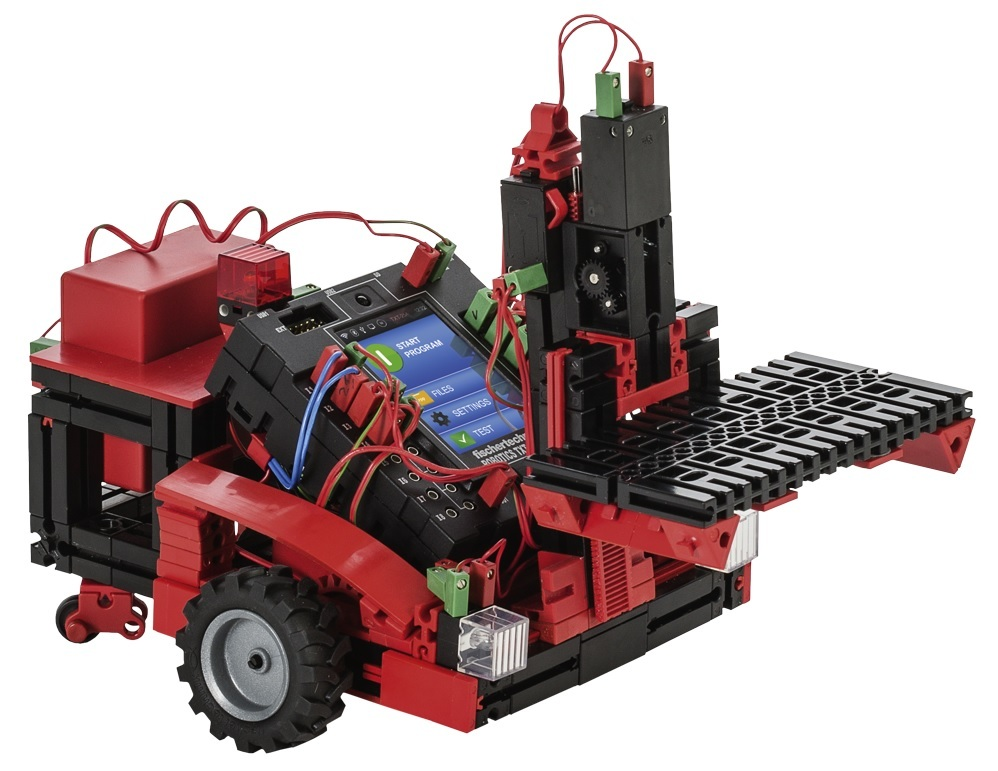
\includegraphics[width=300px]{images/fischertechnik_ROBO-TX-Explorer_02.jpg}
% 	\caption[Fischertechnik - ROBO TX Explorer]{Fischertechnik - ROBO TX Explorer \footnote{Zdroj: \url{http://www.helago-cz.cz/eshop-519143-workstation-robo-tx-training-lab-tx-explorer-146560.html}}
% \end{minipage}
% \end{figure}

% figure + footnote -> afterpage
% src: http://tex.stackexchange.com/questions/10181/using-footnote-in-a-figures-caption
%\afterpage{
%	\begin{figure}[h]
%	 	\centering
%		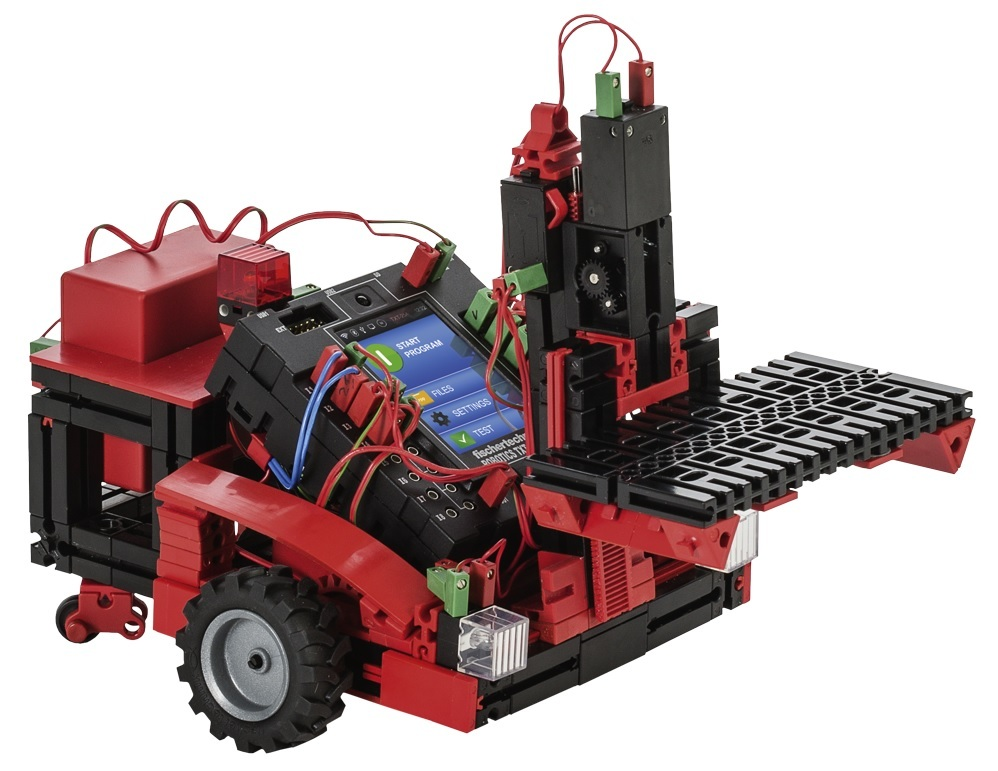
\includegraphics[width=300px]{images/fischertechnik_ROBO-TX-Explorer_02.jpg}
%			\caption[Fischertechnik - ROBO TX Explorer]{Fischertechnik - ROBO TX Explorer \footnotemark}
%		\label{fig:fischertechnik_ROBO-TX-Explorer}
%	\end{figure}
%	\footnotetext{Zdroj: \url{http://www.helago-cz.cz/eshop-519143-workstation-robo-tx-training-lab-tx-explorer-146560.html}}
%}

\begin{figure}[h]
	\centering
	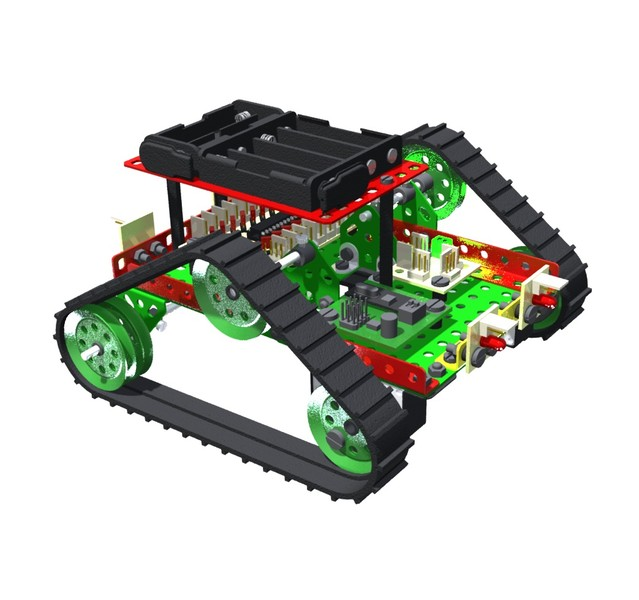
\includegraphics[width=235px]{images/MERKUR_Pasovy-podvozek-01_ATMEL+RC.jpg}
	\caption[MERKUR -- Pásový podvozek 01 -- ATMEL + RC]{MERKUR -- Pásový podvozek 01 -- ATMEL + RC\protect\footnotemark}
	\label{fig:MERKUR_Pasovy-podvozek-01_ATMEL+RC}
\end{figure}

\footnotetext{Zdroj: \url{http://www.merkurtoys.cz/vyrobky/pasovy-podvozek-merkur-s-elektronikou-rc}} 

Další zajímavou stavebnicí jsou Robotické sety od \merkur{u}~\cite{merkur_roboticsSetsEshop}. 
Nabídka jednotlivých setů je relativně široká a~v~porovnání s~\legoM{ }nebo \fischerT{ }nabízí ještě bližší kontakt s~elektronikou a~samotným hardwarem. 
Jako řídicí mikrokontroléry můžete využít PIC nebo megaAVR od firmy Microchip. 

Vzhledem k~použitým procesorům je možné tyto stroje programovat v~C/C++, PICAXE BASIC nebo i~v~grafickém prostředí~\cite{picaxeCz_BlocklyForPICAXE}. 
Robotické stavebnice od Merkuru mají podobné \uv{problémy} jako \fischerT. 
Kladou na uživatele větší nároky, nemají tak zvučnou značku, mají omezenější základní sadu senzorů a~neumožňují tak rychlou stavbu fungujícího robota.

Na závěr lze zmínit výukové roboty, kteří jsou primárně, na rozdíl od robotických stavebnic, zaměřeny na velmi úzkou oblast činností (jízda po čáře, plnění jednoduchých sekvenčních úkolů, \dots). 
Tyto roboty jsou zajímavé z~pohledu ceny, ale i~jednoduššího využití ve výuce (žáci nemusí sestavovat konstrukci a hardware je plně připraven k~používání). 

Naopak již neumožňují rozvoj kreativity studentů při stavbě a přizpůsobení robota pro různé soutěže (většinou je lze využívat jen v~jedné soutěžní kategorii).  
Mezi takovéto roboty patří například Pololu~3pi~\cite{robotPololu3pi} (primárně určen pro jízdu po čáře -- zvládá jezdit až~1~m/s) nebo Edison~\cite{robotEdison} (umí sledovat čáru, lze jej programovat graficky i~v~Pythonu, má různé senzory, je možné jej kombinovat s~\lego{ }kostkami). 

Tyto roboty ovšem neumožňují takový rozsah činností jako \legoM.

\begin{figure}[h]
	\begin{minipage}[b]{.5\textwidth}
		\centering
		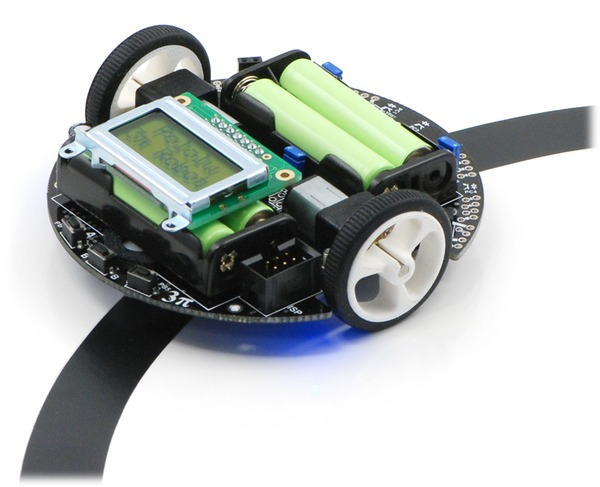
\includegraphics[width=\textwidth]{images/pololu-3pi-robot-8-on-line.jpg}
		\caption[Robot Pololu 3pi]{Robot Pololu 3pi\protect\footnotemark}
		\label{fig:pololu-3pi-robot-8-on-line}
	\end{minipage}
	\hfill
	\begin{minipage}[b]{.5\textwidth}
		\centering
		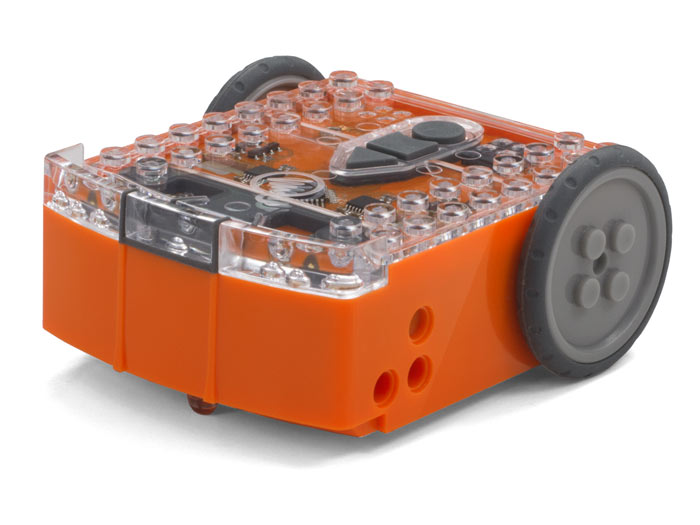
\includegraphics[width=\textwidth]{images/Edison-Educational-robot.jpg}
		\caption[Robot Edison]{Robot Edison\protect\footnotemark}
		\label{fig:Edison-Educational-robot}
	\end{minipage}
\end{figure}

% two footnote/footnotemark in minipage - problem with index
% solution: http://tex.stackexchange.com/a/43694

\addtocounter{footnote}{-1} % footnote_cnt -= 1
\footnotetext{Zdroj: \url{https://www.pololu.com/product/975}}
\stepcounter{footnote}
\footnotetext{Zdroj: \url{https://meetedison.com/meet-edison-v2-0/}}


% putting two images beside each other
% source: http://tex.stackexchange.com/a/148445

%\begin{figure}[!tbp]
%	\begin{subfigure}[b]{.5\textwidth}
%		\centering
%		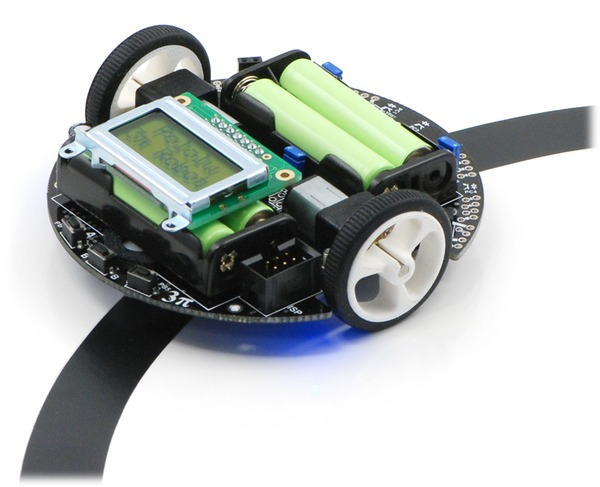
\includegraphics[width=\textwidth]{images/pololu-3pi-robot-8-on-line.jpg}
%		\caption[Robot Pololu 3pi]{Robot Pololu 3pi\protect\footnotemark}
%		\label{fig:pololu-3pi-robot-8-on-line}
%	\end{subfigure}
%	\hfill
%	\begin{subfigure}[b]{.5\textwidth}
%		\centering
%		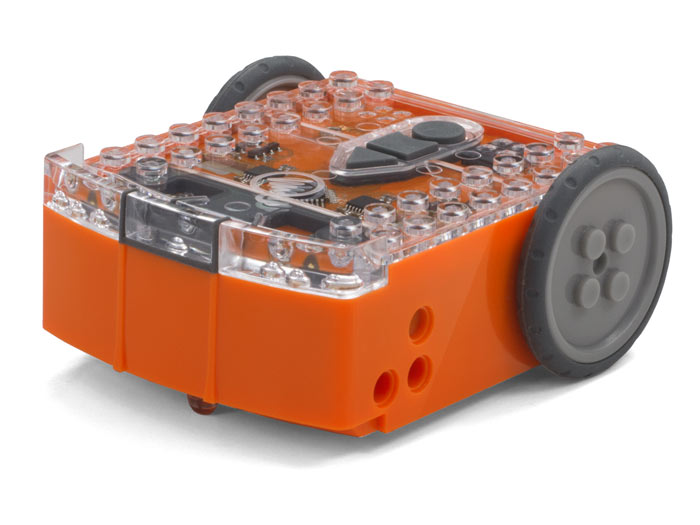
\includegraphics[width=\textwidth]{images/Edison-Educational-robot.jpg}
%		\caption[Robot Edison]{Robot Edison\protect\footnotemark}
%		\label{fig:Edison-Educational-robot}
%	\end{subfigure}
%	\caption{Roboti se zaměřením na velmi úzkou oblast činnost}
%\end{figure}
%
%\footnotetext{Zdroj: \url{https://www.pololu.com/product/975}} 
%\footnotetext{Zdroj: \url{https://meetedison.com/meet-edison-v2-0/}} 

\section{Motivace autora}

Již čtvrtým rokem vedu robotický kroužek na své bývalé střední škole SPŠ a VOŠ Brno, Sokolská a~zároveň organizuji tábory a~další vzdělávací akce v~oblasti techniky a~robotiky na pobočce Robotárna, Dům děti a~mládeže Brno, Helceletova.
Už na střední škole jsem se v~rámci těchto dvou organizací účastnil různých soutěží, jako například Robotický den v~Praze, Mikrokontroléry letí na FEKT VUT Brno nebo Středoškolská odborná činnost (obory strojírenství a~elektrotechnika). 
Z~některých soutěží jsem si dovezl cenná umístění, ale~i~mnoho zkušeností, inspirace a~podnětů na přemýšlení.


Za dobu, kterou se věnuji programování mikrokontrolérů a~robotice, jsem již narazil na mnoho překážek a~problémů, které bylo třeba překonat. 
%si už mnohokrát prošel trnitou cestou 
Tyto překážky jsou ovšem výrazně náročnější pro studenty, kteří v~těchto oblastech teprve začínají a~seznamují se s~nimi. 

Často může nastat i~situace, kdy je student se zájmem o~robotiku odrazen její počáteční složitostí.

Přitom by z~něj mohl být v~budoucnu perfektní programátor. 
Jen mu zrovna tenhle mikrokontrolér nejde naprogramovat nebo mu koupený H-můstek nechce roztočit motor.

Proto se svým studentům vždy snažím nachystat co nejlepší prostředí pro začátky s~robotikou. 

Již jsem zkoušel různé platformy (například využít k~výuce robota Pololu~3pi) i~způsoby výuky (kombinace elektroniky, programování na PC a~programování mikrokontrolérů), ale~bohužel vždy jsem se dostal do stejné situace. 

Ačkoliv mi studenti chodili již rok do robotického kroužku, pořád je dělily minimálně dva roky od schopnosti postavit a~naprogramovat složitějšího robota (s~tím, že by použili předpřipravenou elektroniku, ale rozuměli tomu, co je jak zapojeno + uměli použít dostupné knihovny a~naprogramovat si chování svého robota).

Nedávno jsme ale do kroužku zakoupili \legoEV{}. 
Stavebnici, která mi měla umožnit postavit robota za den. 
Prakticky stavebnice snů. No není to nádherná představa?
A~opravdu tomu tak bylo. Robota jezdícího po čáře jsme s~manuálem zvládli poskládat a~zprovoznit za den. 
Studenti nemuseli studovat a~řešit zapojení jednotlivých komponentů do řídicí elektroniky. 

Nebylo třeba trávit mnoho času vysvětlováním způsobu programování 8bitových mikrokontrolérů (omezení paměti a~výkonu, menší datové typy -- \verb|uint_8t|, komunikace po sériové lince, \dots).

Jen si poskládali z~\lega{ }hardware, pomocí kabelů (které nelze otočit ani zapojit špatně a~tím něco zničit) spojili jednotlivé moduly. 

A~v~grafickém prostředí si poskládali svůj program.

Pak jsme se ale začali soustředit na zlepšování softwaru i~hardwaru tak, abychom využili stavebnici na 100~procent, a~v~ten moment jsme narazili.

Dokud jsme si s~EV3 jen \uv{hráli} a~nesoustředili se primárně na výkon a~spolehlivost, bylo vše v~pořádku. 
Jakmile jsme ale chtěli mít regulační smyčku PID~regulace pro robota na sledování černé čáry s~periodou 10~ms, zjistili jsme, že to nejde (a~to máme v~EV3 \brick{\it u} 300~MHz~ARM). Přitom díky předešlým zkušenostem s~8bitovými mikrokontroléry Atmel~AVR jsme věděli, že by to neměl být problém.


To samé platí o~grafickém vývojovém prostředí dodávaném s~\EVthree. Dokud máte na obrazovce několik programových bloků, vše funguje bez problémů. 
Když se však program rozroste na několik obrazovek a~samostatných modulů, velmi rychle ztrácíte přehlednost a~efektivitu programování.
Zároveň vám již moc nepomohou ladicí nástroje, které jsou součástí prostředí, protože při jednoduchém programu je lze relativně dobře využít, ale při rozsáhlejších programech již nejsou k~dispozici nebo je jejich použití velmi komplikované. 


Proto jsme začali hledat alternativní platformy, které by odstraňovaly zmíněné problémy, což vyústilo v~tuto práci.   

